\documentclass[16pt,a4paper]{report}
\usepackage[utf8]{inputenc}
\usepackage{graphicx}
\usepackage{geometry}
\usepackage{dirtytalk}
\usepackage{array}
\usepackage{hyperref}
\usepackage{setspace}
\usepackage{float}
\hypersetup{colorlinks=true, linkcolor=black}
\usepackage{fixltx2e}
\usepackage{graphicx}
\usepackage{amsmath}
\usepackage{amssymb}
\usepackage{latexsym}
\usepackage{siunitx}
\usepackage{graphics}

\usepackage{silence}
\WarningFilter{latex}{Command \InputIfFileExists}
\usepackage{fontspec}

%%% For language switching -- like babel, but for xelatex
\usepackage{polyglossia}

\setmainlanguage{english}
\setotherlanguages{hindi,sanskrit} %% or other languages

\newfontfamily\devanagarifont[Script=Devanagari]{Lohit Devanagari}

\usepackage[boxed]{algorithm2e}
% \usepackage[nottoc]{tocbibind}
\usepackage[nottoc,notlof,notlot]{tocbibind} 
\renewcommand\bibname{References}  % to rename bibliography to reference
\usepackage[document]{ragged2e}
\bibliographystyle{plain}
% \title{SeminarReport}
% \author{anand.nitb19 }
% \date{April 2017}
%\geometry{margin=1in}
\begin{document}
%\setstretch{1.5}
\begin{center}
    \rule[0.5ex]{\linewidth}{2pt}\vspace*{-\baselineskip}\vspace*{3.2pt}
    \rule[0.5ex]{\linewidth}{1pt}\\[\baselineskip]
    {\LARGE Machine Translation and its Evaluation }\\[2mm]
    \rule[0.5ex]{\linewidth}{1pt}\vspace*{-\baselineskip}\vspace{3.2pt}
    \rule[0.5ex]{\linewidth}{2pt}\\
    \vspace{6.5mm}
    {\large \textbf{A Seminar Report}}\\[5pt]
    {\large \textit{Submitted in partial fulfillment of requirements for the degree of}}\\[5pt]
    {\large \textbf{Master of Technology}}\\
    \vspace{6.5mm}
    {\large By}\\
    \vspace{3mm}
    {\large\textbf{Anand Namdev}}\\
    {\large\textbf{Roll Num: 163050068}}\\
    \vspace{6.5mm}
    {\large \textit{under the guidance of }}\\[5pt]
    {\large\textbf{Prof. Pushpak Bhattacharyya}}\\
    \vspace{11mm}
    
\includegraphics[scale=0.6]{Images/iitblogo.jpeg}\\
    \vspace{6mm}
    {\large Department of Computer Science and Engineering\\
    \textsc{Indian Institute of Technology, Bombay}}\\
    \vspace{11mm}
    \vspace{9mm}
    {\large\textsc{April, 2017}}
    \vspace{12mm}
\end{center}

\newpage
\begin{center}
    \section*{\textbf{\LARGE Acknowledgement}}
    \justify
    I am extremely thankful to my seminar guide \textbf{Prof. Pushpak Bhattacharrya} for helping me through out the research seminar. All the seminar meetings have been very crucial in resolving doubts related to the Machine Translation. I can't thank enough my parents for their constant encouragement and support. I am also very grateful to my peers \textbf{Sanket Gandhare} and \textbf{Ajay Gupta} for all the discussions held through out the semester. 
\end{center}

\newpage
\begin{center}
    \section*{\textbf{\LARGE Abstract}}
    \justify
    Natural Language Processing is one of the branch of Artificial Intelligence which involves large amount of processing of human language. Machine Translation is one of the most prominent problem of Natural Language Processing. It is a old and an important machine learning, because there is large amount of data which can't be translated by human translators. It has evolved from traditional Rule based Machine Translation (RBMT) to Statistical Machine Translation (SMT) to very sophisticated Neural Machine Translation (NMT). This seminar reports explores the types of machine translation techniques used, the pros and cons of using any method and finally the evaluation of a Machine Translation System.
\end{center}
 


    \tableofcontents
    \addcontentsline{toc}{section}{Acknowledgement}
    \addcontentsline{toc}{section}{Abstract}
    \newpage
    \listoffigures
    \newpage
    \listoftables
    \newpage
    \chapter{Introduction}
\section{Machine Translation}
    \justify
    \textbf{Machine Translation}, which is also abbreviated by \textbf{MT} is an important problem of Natural Language Processing (NLP). It can be defined as- \say{the translation of human language by a machine}. The machines are trained in such a way that, during testing, it can translate any text from a \textit{source language} to \textit{target language}. \textit{Source language} is the language in which a text is already written; while \textit{target language} is the language in which text has to be translated. 
    
\section{History of Machine Translation}
    The current \textit{state-of-art} MT researchers have made very sophisticated MT systems capable of translating a text with very good accuracy, giving almost 100\% knowledge about the sentence. But the main research in the field MT began in 1950s. \textbf{The Georgetown Experiment}\cite{MThistory} was the earliest MT experiment, which involved translating 60 Russian sentences into English. 
    
    The earlier systems consisted of a bilingual dictionary which had a mapping for each word from source language to target language and set of rules to predict word order once all words were mapped. This systems were too constrained in the sense that they were language specific, rules change as the target or source language change, the rules were not even consistent as there were always sentences which didn't follow the grammar rules. There was a clear lack of semantic rules which could actually grasp the meaning of sentence. Researchers in time couldn't find specific solutions for such problems. This led to the shutting down funding in the research of MT by ALPAC committee\cite{MThistory} in 1964 formed by US government. 
    
    The 1980s and 90s saw the rise of many MT based systems namely \textbf{Systran} and \textbf{Logos}, which translated text to/from German, Russian and other European languages. Several Example Based Systems were also developed in the same period, in which for each source sentence, the most similar sentence in target language was found in parallel corpus. Meanwhile, data driven methods began popularity. IBM began its research in MT with a more specific term called as \textbf{Statistical Machine Translation}. Currently, SMT is one of the most sutdied MT method. Various IBM model were released sequentially to overcome the drawback of previous models. Later on an MT engine based on SMT called \textbf{Moses} was also released. 
    
    \begin{figure}
        \centering
        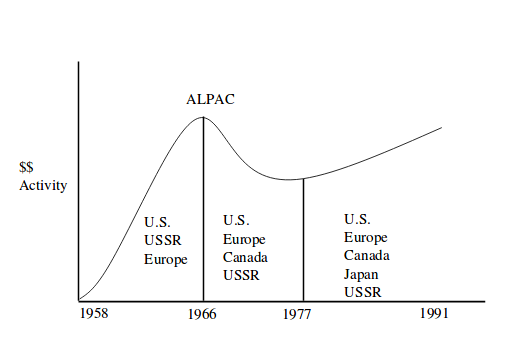
\includegraphics[scale=0.6]{Images/mtHistory.png}
        \caption{History of MT}
        \label{fig:history}
    \end{figure}
    The state-of-the art method used primarily in MT is Neural Machine Translation, which uses Neural Networks to encode source sentences to decode in target sentences. Currently, an open source Neural Networks based Machine Translation system is developed by Harvard known as OpenNMT\cite{openNMT}.
        
\section{Paradigms of Machine Translation}
    The three main paradigms of Machine Translation are Rule Based Machine Translation, Statistical Machine Translation and Example Based Machine Translation. The main goal of all the paradigms are the same, i.e. to translate a text from source to target language. However, all the paradigms differ in the methodology of translating. Each paradigm has its own pros and cons of using it, like the domain, cost to build such a system, time to build and most importantly the accuracy of the translation.
    
    \subsection{Rule Based Machine Translation}
    \textbf{Rule Based Machine Translation} or more commonly known as \textbf{RBMT} is a traditional paradigm of machine translation. It uses the linguistic information of the language to create rules using which it helps in translation. Since the whole idea of translation in this paradigm is based on rules of language, hence rules should be carefully written. Rules are written by linguistic experts of languages which are involved in translation. All the diverse phenomenon should be covered by rules of the translation. 
    
    Rule based MT incurs huge time and effort. Each phenomena of the language has to be captured which is generally not possible. Rule based MT often suffers from high precision and low recall problem, i.e. the system will perform good on seen data since seeing them rules are written by the expert, but will perform poorly on unseen data. The diverse language regularities and constraints are often uncovered by rules.
    
    \subsection{Statistical Machine Translation}
    \textbf{Statistical Machine Translation} or \textbf{SMT} is a data-driven method of Machine Translation. Unlike RBMT, there are no rules in SMT, instead a thorough statistical analysis of parallel corpora has to be done. IBM began research in SMT, developing various SMT models called as the IBM models. Each model captures a distinct feature of language and overcomes drawbacks of previous models. 
    
    Statistical Machine Translation does translation by capturing probabilities of two models, namely \textbf{Translational Model} and \textbf{Language Model}. Translational models gives the probability of how likely is the target sentence given source sentence, which is often broken down to word level. Language model gives the probability of how probable is the translated target language sentence with respect to fluency and adequacy in the context of target language sentence. Both these probabilities are combined to form a noisy-channel model which predicts the most probable sentence from a source language sentence.
    
    \subsection{Example Based Machine Translation}
    \textbf{Example Baed Machine Translation} or \textbf{EMBT} is another paradigm of machine translation. It was introduced in 1980s. 
    
    EBMT is also a data-driven method, it heavily depends on parallel corpora. A source language sentence is searched in the parallel corpora to find best possible matching sentence in source language. If an exact match is found, then its translation in the target language which is also stored in parallel corpora is returned. But if no exact match is found, best possible matching sentence is taken and it's translation is returned with slight modifications to the translation to adapt the changes. Sometimes two or more sentence are matched in parts, and their translations are returned and joined in similar fashion to return one single translation of the source sentence. 
    
    

    \chapter{Rule Based Machine Translation}
\section{Understanding RBMT}
    Rule Based Machine Translation is one of the earliest paradigm of Machine Translation. Rules are written to translate a text from source language to target language. A typical translation in any paradigm of Machine Translation is a 3-step, \textit{Analysis-Transfer-Generation (ATG)} process. It is the transfer phase of Translation which is most important for each paradigm. For instance, in the case of RBMT, transfer takes place through human created rules.
    
    However, Pure RBMT would use rules at every stage of ATG process\cite{bhattacharyya}:
    
    \begin{enumerate}
        \item During analysis, RBMT would use rules to analysis and recognize various features, ambiguities present in the text. A typical text in natural language contains many different ambiguities like\cite{NLPAmbiguity}:
        
        \begin{itemize}
            \item Lexical Ambiguity: Ambiguity of a single word. Ex: book
            \begin{flushleft}
            book(NN): CLRS is the foundation book in Algorithms.\linebreak
            book(VB): Book a return ticket to Delhi.\linebreak
            \end{flushleft}
            
            \item Lexical Semantic Ambiguity: When a single word is used in multiple senses. Ex: Tank
            \begin{flushleft}
            The water tank is full of Water. \linebreak
            I saw a military tank.
            \end{flushleft}
            
            \item Scope Ambiguity: Ambiguity about score of words
            \begin{flushleft}
            Ex: Poor boys and girls should have a right to study.\linebreak
            Poor (boys and girl) or (Poor boys) and girls
            \end{flushleft}
            
            \item Attachment Ambiguity: Ambiguity about attaching a phrase in sentence
            \begin{flushleft}
            I saw a boy running.\linebreak
            Who was running? I or the boy.
            \end{flushleft}
            
            \item Discourse: Ambiguity about attaching a word to its parent in the previous sentence.
            \begin{flushleft}
            Ram was a good friend of Shyam. He never betrayed him.\linebreak 
            He and him refers to who? Ram or Shyam
            \end{flushleft}
            
            \item Pragmatics: Situation where context of a phrase gives multiple iterpretations.
            \begin{flushleft}
            I love you too.\cite{sep-ambiguity}\linebreak 
            This can be interpreted as:\linebreak 
            I love you (just like you love me)\linebreak 
            I love you (just like someone else does)\linebreak 
            I love you (and I love someone else)\linebreak 
            I love you (as well as liking you)\linebreak 
            \end{flushleft}
        \end{itemize}    
        There are various many other ambiguities that can be find in a Natural Language  like boundary ambiguity, morphological features ambiguity, named entity vs common noun ambiguity etc. Depending on the depth of analysis, rules are written to capture the above situations.
        
        \item During transfer, a bilingual mapping or dictionary look-up for each word of source sentence is done. If the analysis step is precisely done, then this step is easy since analysis step removes most of the disambiguation from the language.
        
        \item During generation, RBMT would arrange all the mapped words of target language that were obtained from bilingual mapping and perform syntax ordering, i.e. place words according to the syntactic rules of target language. 
            
    \end{enumerate}

\section{The Two kinds of RBMT: Interlingua and Transfer} 
    \subsection{Understanding Interlingua}
    An interlingua can be defined as the ultimate knowledge source. It is itself a language in the sense that it contains the representation of any language in most disambiguated form. An interlingua is artificial and is created by linguistic experts for the purpose of representing meaning in a computer. 
    \begin{figure}
        \centering
        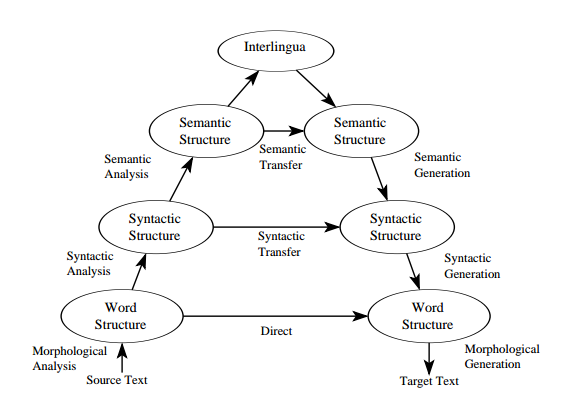
\includegraphics[scale=0.6]{Images/interlingua.png}
        \caption{Vauquois Triangle: Approaches to Machine Translation}
        \label{fig:triangle}
    \end{figure}
    
    Fig.\ref{fig:triangle}\cite{dorr} explains the approaches to MT. The higher one goes on the upward hill, the most complex is the representation. Interlingua is at the top of the figure, implies that the representation is really difficult to obtain with all the attributes in its disambiguated form. However, once the Interlingua is made, translation to target language is equally easy.
    
    So given a sentence, its interlingual representation would include the following\cite{bhattacharyya}:
    \begin{enumerate}
        \item Lexical Knowledge
        \item Structural Knowledge
        \item Discourse Knowledge
    \end{enumerate}
    
    This means its interlingual representation would include\cite{bhattacharyya}:
    \begin{enumerate}
        \item All the words in disambiguate form
        \item All words groups like multiwords
        \item All Structural ambiguities like attachment 
        \item All Discourse ambiguities like co-reference
    \end{enumerate}
    
    \subsection{Universal Networking Language (UNL): A type of Interlingua}
    UNL is an interlingua that represents information sentence by sentence. A hypergraph is made for each sentence with concepts as nodes and relations as arcs. The knowledge is primarily represented in 3-dimensions.
    \begin{enumerate}
        \item \textbf{Word Knowledge} is represented by Universal Words or UWs that are language independent. UWs are picked from lexicon during analysis phase. UWs also contains restrictions that correctly disambiguate the meaning of word. Ex: \textit{drink(icl$>$liquor)} denotes the Noun \textit{liquor}. The \textit{icl} notation indicates `inclusion' and forms an \textit{is-a} relationship.
        
        \item \textbf{Conceptual knowledge} is represented by forming a binary relation between UWs through \textit{relation labels}. There are about \num{46} relation label in UNL. A relation is typically represented as \textit{rel(UW1,UW2)}.
        
        \item Speaker's view, aspect and time are captured by attribute labels.
    \end{enumerate}
    
    \subsection{Illustration of UNL}
    \subsection{Challenges to UNL and Solution}
    Interlinguas is a universal representation of all languages as we have seen. But an important question arises. Is this knowledge repository possible? 
    \subsection{Translation Using Interlingua}
    For translation using Interlingua, only the steps of ATG process are required, since there is no transfer involved in Interlingua. First, a thorough analysis of source sentence is done to create Interlingua (A-Stage). Secondly, target sentence is generated in G-stage using syntax planning, word-ordering and functional word insertion.
    
    A sample example from \cite{bhattacharyya} is shown here to present how translation works in UNL.
    
    \begin{flushleft}
    E: On Sunday in Kolkata, Sachin donated to the cricket museum the bat with which he scored his hundredth century at Bangladesh.\\
    H: 
    \begin{hindi}
    रविवार को कोलकाता मे सचिन ने क्रि्केत सन्ग्रहलय को वह बल्ला दान कर दिया जिससे उन्होने बान्ग्लादेश मे अपना सौवा शतक लगाया| \\
    \end{hindi}
    HT: ravivaar ko kolkata mein sachin ne kriket saMgrahaalaya ko vaha ballaa daan kar diyaa jisase unhone Bangladesh mein apnaa sauwaan shatak lagaayaa thaa.
    \end{flushleft}
    
    \begin{figure}
        \centering
        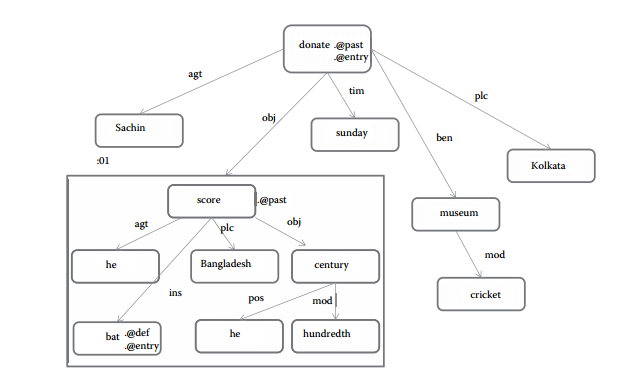
\includegraphics[scale=0.6]{Images/unl}
        \caption{UNL graph for example sentence.}
        \label{fig:unl}
    \end{figure}
    The analysis stage will:
    \begin{enumerate}
    \item Recognize named entities: Sachine(Person), Kolkata(location), Bangladesh(location)
    
    \item POS of words: On/IN Sunday/NNP in/IN Kolkata/NNP,/, Sachin/NNP donated/VBD to/TO the/DT cricket/NN museum/NN the/DT bat/NN with/IN which/WDT he/PRP scored/VBD his/PRP hundredth/JJ century/NN at/IN Bangladesh/NNP
  
    \item Get morphological information of words, i.e. \textit{donate}- main verb, past tense
    
    \item Get sense IDs of words through word sense disambiguation, i.e. \textit{donate(icl$>$give$>$do,agt$>$thing,obj$>$thing)}.
    
    \item Establish semantic relations between verb and noun, i.e. \textit{nsubj(donated-7, Sachin-6)}
    
    \item Generate attributes using grammatical properties, i.e. add .@entry and .@past attributes on donate.
    \end{enumerate}
    
    Similarly the generation stage will contain the following steps:
    \begin{enumerate}
    \item The graph corresponding to Fig.\ref{fig:unl} is parsed to record headwords, IDs, attributes and semantic relations.
    
    \item Do appropriate word mapping from lexicon. Eg: \textit{donate} $\leftrightarrow$ \textit{daan karnaa}.
    
    \item Identify case-markers for words. Eg: \textit{Kartaa Kaarak} for Sachine.
    
    \item Morphological Synthesis of words. Eg: \textit{daan karnaa} $\leftrightarrow$ \textit{daan kar diyaa}.
    
    \item Function word generation. Eg: \textit{ne} for noun Sachin, \textit{ko} for samgrahaalaya.
    \end{enumerate}
    
    \subsection{Transfer-Based MT}
    Transfer based MT is a explicit source-target pair MT, where rules are written with only source and target language in mind. It also does not insist on complete disambiguation of source sentence. 
    
    Transfer rules are typically structural transforming rules applied between a pair of languages. Transfer rules can't be generalized with any other pair of language, since they are written explicitly for each pair at a time. A transformation T can be written as\cite{bhattacharyya}:
    \begin{equation}
    T: REP_s \rightarrow REP_t
    \end{equation}
    where $REP_s$ and $REP_t$ are source and target language representation respectively. \linebreak
    Eg: E: I go to school. \\
    \quad H:
        \begin{hindi}
        मै विद्यालय जाता हूँ |\\
        \end{hindi}
       For the above example, the rules can be of the type
       \begin{equation}
    T: SVO \rightarrow SOV 
    \end{equation}
    i.e. the object and verb of the sentence should be swapped to get desired Hindi sentence output.
        
    
   	
    
    \chapter{Statistical Machine Translation}
\label{chap:SMT}
\section{Motivation behind SMT}
	\textbf{SMT} unlike RBMT doesn't depend on complex rules to translate from source language to target language. Also, rules are written with keeping a pair of language in mind, hence can't be generalized over other pairs. SMT on the other hand relies heavily on availability of parallel corpora. There is no dependency on pair of language involved in translation. 	

\section{Noisy Channel Model of Translation}
SMT is based on simple Noisy channel model. For instance in the case of Foreign (\textit{f}) $\rightarrow$ English (\textit{e}), the posterior probability of most likely English sentence given the foreign sentence can be broken product of most likely foreign sentence given the English sentence and prior of English sentence. The above hypothesis can be written in equation as:-\\
\begin{equation}
\hat{e} = arg max_{e}(P(e\mid f)) = arg max_{e}(P(e)\cdot(f\mid e))
\end{equation}
where $P(f\mid e)$ is called the translation model and $P(e)$ is called the language model.

\subsection{Lexical Translation of Words}
Translation model can be thought as translating each word of the foreign sentence with the most likely word in the source language. This type of estimating the translation for each word is called as Maximum likelihood estimation.\\
For ex: What is the most likely English translation for a foreign word like \textit{Haus}?\cite{koehn}\\ 
Or to put it in a equation it can be written as\\
\begin{equation}
p_{f}: e \rightarrow p_{f}(e)
\end{equation}
i.e. for a given foreign word $f$, it returns a probability $p_{f}(e)$ depicting how likely is the translation. 
% Also, the function $p_{f}(e)$ must follow two following properties:\\
% \begin{equation}
% \sum_{e}^{}p_{f}(e) = \text{1}
% \forall \textsubscript{e} 0 \leqslant p_{f}(e) \leqslant 1
% \end{equation}
\begin{figure}
        \centering
        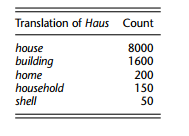
\includegraphics[scale=0.6]{Images/table1}
        \caption{Sample count data}
        \label{fig:count}
\end{figure}
Fig \ref{fig:count} shows count of translation of the word \textit{Haus} in English from \cite{koehn}.\\
Also Eq \ref{eq:3.3} represents the calculated lexical probability of translating the \textit{German} word \textit{Haus} to the following English word. \\

\begin{equation} \label{eq:3.3}
    X=
    \begin{cases}
      0.8, & \text{if e=house}\ \\
      0.16, & \text{if e=building}\ \\
      0.02, & \text{if e=home}\ \\
      0.015, & \text{if e=household}\ \\
      0.005, & \text{if e=shell}\ \\
    \end{cases}
\end{equation}
    
We can apply the above maximum likelihood hypothesis by translating for each foreign word, the English word for which the probability function is maximum. This type of translating a sentence word-by-word is very intuitive but is only useful when languages belong to same family. Because, languages of same families tend to have the same word order which is rarely the case since we always want translation between any pair of languages. Translation between any pair of languages incurs Alignment, which is mentioned in the next section.

\section{Alignment}
A pair of sentence can have the following alignment settings\cite{bhattacharyya}:\\
\begin{enumerate}
\item The source and target language are same family languages that the order of word is entirely same. 
\item The source and target language are not of same family but the sentence follows a pattern that each word from source sentence maps to only 1 word in the target language.
\item A word maps to nothing on the target sentence, i.e. null alignment.
\item Multiple words maps to same word in target sentence.
\item One word maps to multiple word in target sentence.
\item Multiple words map to multiple word in target sentence.
\end{enumerate}

\section{Factors Influencing $P(f\mid e)$}
The translation model probability, $P(f \mid e)$ is dependent on following factors:

\subsection{Alignment factor a}	
The translation probability can be expanded to included Alignmnet factor as
\begin{equation}
P(f\mid e) = \sum_{a}P(f\mid e)
\end{equation}
where a runs parallel to a. For ex Fig\ref{fig:alignment}\cite{bhattacharyya} shows a sample alignment between a e $\leftrightarrow$ f pair. Table\ref{tab:alignment} shows the equivalent alignment vector a for the sample sentence.

\begin{figure}
        \centering
        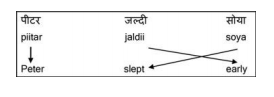
\includegraphics[scale=0.6]{Images/alignment}
        \caption{Alignment between an example e $\leftrightarrow$ f pair.}
        \label{fig:alignment}
\end{figure}



\begin{table}[h!]
\centering
 \caption{Sample alignment} 
 \label{tab:alignment} 
 \begin{tabular}{c c c c} 
 \hline
 Index & 1 & 2 & 3 \\  
 \hline
 F & Piitar & jaldi & soya \\
 a & 1 & 3 & 2 \\ [1ex] 
 \hline
 \end{tabular}
\end{table}

\subsection{Length factor \textit{m}}
Length is also another important criteria for translating sentence. It is used to control or restrict the output. Imagine a translation of a 8-word sentence to be of just 3-words or 20-words. SMT takes this factor into consideration by marginalizing the above \eqref{eq:3.3} with length(m), which becomes:
\begin{equation}
P(f,a\mid e) = \sum_{m}P(f,a,m\mid e)
\end{equation}

Combining the above two factors as together, the translation model becomes\cite{bhattacharyya}


\begin{align*}
P(f,a,m\mid e) &= P(m\mid e)P(f,a\mid e,m) \\
			   &= P(m\mid e)P(f_{1},a_{1},f_{2},a_{2},\ldots,f_{m},a_{m}\mid e,m) \\
               &= P(m\mid e)\prod_{j=1}^{m}P(f_{j},a_{j}\mid f_{1}^{j-1},a_{1}^{j-1},e,m) \\
               &= P(m\mid e)\prod_{j=1}^{m}P(a_{j}\mid f_{1}^{j-1},a_{1}^{j-1},e,m)\prod_{j=1}^{m}P(f_{j}\mid f_{1}^{j-1},a_{1}^{j},e,m) \\ 
\end{align*}
where \\
\begin{itemize}
\item Part1: Length Probability: $P(m\mid e)$ 
\item Part2: Alignment Probability: $\prod_{j=1}^{m}P(a_{j}\mid f_{1}^{j-1},a_{1}^{j-1},e,m)$
\item Part3: Translational Probability: $\prod_{j=1}^{m}P(f_{j}\mid f_{1}^{j-1},a_{1}^{j},e,m)$
\end{itemize}

So, the final Translation model becomes:
\begin{equation}
P(f\mid e) = P(m\mid e)\sum_{a}\Bigg[ \prod_{j=1}^{m}P(a_{j}\mid f_{1}^{j-1},a_{1}^{j-1},e,m)\prod_{j=1}^{m}P(f_{j}\mid f_{1}^{j-1},a_{1}^{j},e,m)\Bigg] 
\end{equation}
the three parts of equation simply means
\begin{enumerate}
\item What is the probability that $e$ generates a sentence $f$ of length m?
\item What is the probability that translation of $j^{th}$ word $f_{j}$ in $f$ would find it's alignment at position $a_{j}$ in $e$?
\item What is the probability that e's translation is $f_{j}$?
\end{enumerate}








    \chapter{IBM models}
\section{Roadmap}
The previous chapter saw the necessary background to study IBM models. This chapter consists of IBM models and their formulations. Each model consists of some assumptions and their assumptions are in the order of increasing complexity. 

The final formulation of translational model as seen in previous chapter was:
\begin{equation}
P(f\mid e) = P(m\mid e)\sum_{a}\Bigg[ \prod_{j=1}^{m}P(a_{j}\mid f_{1}^{j-1},a_{1}^{j-1},e,m)\prod_{j=1}^{m}P(f_{j}\mid f_{1}^{j-1},a_{1}^{j},e,m)\Bigg] 
\end{equation}

\section{IBM model 1}
\subsection{Formulation}
IBM model is most basic model with few assumptions which are
\begin{enumerate}
\item Length of input $m$ and output $l$ is same, i.e. $P(m \mid l) = \epsilon$

\item All alignments are equally likely, i.e. any word in the alignment $a_{j}$ can take 1 out of $(l+1)$ positions with equal probability. So
\begin{equation*}
\prod_{j=1}^{m}P(a_{j}\mid f_{1}^{j-1},a_{1}^{j-1},e,m) =
\frac{1}{(l+1)^m} 
\end{equation*}

\item Any word in the foreign sentence $f_{j}$ depends only on $j^{th}$ word in the alignment $a$ in $e$ which is $e_{aj}$. That is:\\
\begin{equation*}
\prod_{j=1}^{m}P(f_{j}\mid f_{1}^{j-1},a_{1}^{j},e,m) = \prod_{j=1}^{m}P(f_{j}\mid e_{aj})
\end{equation*}
\end{enumerate}
Considering all the three above assumptions and applying optimization steps, the IBM model-1 becomes
\begin{equation}
P(f\mid e) = \frac{\epsilon}{(l+1)^m}\prod_{j=1}^{m}\sum_{i=0}^{l}P(f_{j}\mid e_{aj})
\end{equation}


\subsection{EM for computing $P(f\mid e)$}
\subsection{Decoding in IBM model 1}
Translating a new sentence, once is model is made is called \textit{Decoding}. We apply the same Noisy-channel modal for any new sentence $f^{new}$ as

\begin{align*}
e^{best} &= argmax_{e^{new}}(P(e^{new})P(f^{new}\mid e^{new}))\\
         &= argmax_{e^{new}}\Bigg(P(e^{new})\cdot \frac{\epsilon}{(l+1)^{m}}\sum_{a}\prod_{j=1}^{m}P(f_{j}^{new}\mid e_{a_{j}}^{new})\Bigg) \\
         &= argmax_{e^{new}}\Bigg(P(e^{new})\cdot \frac{\epsilon}{(l+1)^{m}}\prod_{j=1}^{m}\sum_{i=0}^{l}P(f_{j}^{new}\mid e_{a_{j}}^{new})\Bigg) \\
         &= argmax_{e^{new}}\Bigg(\frac{\epsilon}{(l+1)^{m}}\Bigg)\cdot \big(P(e_{0}^{new}) \big)\cdot \Bigg(\prod_{i=1}^{l}P(e_{i}^{new}\mid e_{i-1}^{new})\Bigg)\cdot \Bigg(\prod_{j=1}^{m}\sum_{i=0}^{l}P(f_{j}^{new}\mid e_{a_{j}}^{new})\Bigg) \\ 
\end{align*}

IBM model is the simplest SMT model and has certain loopholes like
\begin{itemize}
\item Length of input and output are considered to be same which is very rare in real scenarios.
\item All the alignments are considered equally likely i.e. any word $e_{j}$ in $e$ can come at any position in $f$ which is again very naive.
\item For each word there is exactly 1 word associated with it. There are no null or multiple alignments.
\end{itemize}

This led to future IBM models.

\section{IBM model 2}
IBM model II has a two step process i.e. it has a lexical translation step which translates each word of the $f$ into $e$ and then the alignment step which does alignment on each word of $e$
\subsection{Formulation}
IBM model-2 takes certain assumptions into account like
\begin{enumerate}
\item Takes alignment into consideration i.e.
\begin{equation*}
\prod_{j=1}^{m}P(a_{j}\mid f_{1}^{j-1},a_{1}^{j-1},e,m) = \prod_{j=1}^{m}P(a_{j}\mid j,l,m)
\end{equation*}
\item $f_{j}$ depends on $e_{a_{j}}$ so,
\begin{equation*}
\prod_{j=1}^{m}P(f_{j}\mid f_{1}^{j-1},a_{1}^{j},e,m) = \prod_{j=1}^{m}P(f_{j}\mid e_{aj})
\end{equation*}
\end{enumerate}
So the translation model becomes,
\begin{equation}
P(f\mid e) = \epsilon\prod_{j=1}^{m}\sum_{i=0}^{l}P(i\mid j,l,m)P(f_{j}\mid e_{i})
\end{equation}

Again, IBM model II is not the best of the SMT model and has following loopholes
\begin{itemize}
\item Length of input and output are considered to be same which is too ideal.
\item No null and multiple alignments for a word, each word has exactly 1 alignment.
\end{itemize}

\section{IBM model 3}
So far IBM model didn't model number of words produced from any foreign sentence word. IBM model models this feature using fertility.

Fertility $n(\phi \mid f)$ can be defined as for each foreign word number of words $\phi = 0,1,2,\cdots$ generated. Words can be handled by considering $\phi=0$.
Also, word insertion can be modeled by considering $n(\phi \mid NULL)$.

Translation by IBM model III is a four step model which is explained by an example \ref{fig:4steps} from \cite{koehn}:
\begin{figure}[H]
        \centering
        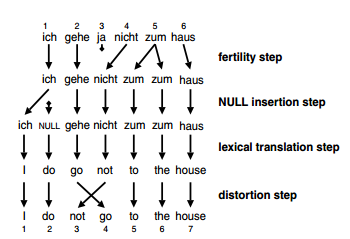
\includegraphics[scale=0.6]{Images/4steps}
        \caption{4 steps of IBM model III}
        \label{fig:4steps}
\end{figure}
\begin{enumerate}
\item Fertility Step: For each word $s_{i}$ of source sentence s, fertility $\phi_{i}$ is chosen with probability $P(\phi_{i}\mid e_{i})$.
\item Null Insertion Step: Number of target words to be generated from \textit{NULL} is chosen with probability $n(\phi \mid NULL)$.
\item Lexical Translation Step: Translation of each word similar to IBM model I is done by $P(e\mid f)$.
\item Distortion step: Probability of translating a $i_{th}$ positioned foreign word $f_{i}$ as $j_{th}$ positioned source word $s_{j}$ is modeled by $d(j\mid i,l,m)$.
\end{enumerate}

IBM model doesn't consider Alignment rather the same phenomena is captured by distortion probability. The reason being, since IBM model III introduces fertility, a single word can be broken into multiple words. Those multiple words can be rearranged into many permutations, but all those permutations will have the same alignment probability since the alignment vector for all those permutations will be entirely the same. Fig \ref{fig:distortion} explains this effect clearly,
\begin{figure}[H]
        \centering
        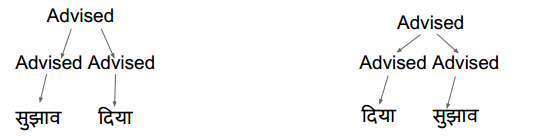
\includegraphics[scale=0.6]{Images/distortion}
        \caption{Sample example to show difference between alignment and distortion}
        \label{fig:distortion}
\end{figure}

Hence the equation for IBM model III becomes
\begin{align}
P(f\mid e) &= \sum_{a_{1}}^{l}\ldots \sum_{a_{m}}^{l}\nonumber \\
		   &= \sum_{a_{1}}^{l}\ldots \sum_{a_{m}}^{l}\binom{m-\phi_{0}}{\phi_{0}}p_{0}^{m-2\phi_{0}}p_{1}^{\phi_{0}}\prod_{i=1}^{l}\phi_{i}!n(\phi_{i}\mid e_{i})\times \prod_{j=1}^{m}t(f_{j}\mid e_{a_{j}})\mid d(j\mid a_{j},m,l)
\end{align}

IBM model III is a very strong SMT model. However, it also has certain complexity issues like
\begin{itemize}
\item When value of $m$ and $l$ are huge, the distortion matrix will be very sparse and most of the values will be zeros. It doesn't take into effect that words(phrases) that are together in the input tend to be together in the output.
\end{itemize}





















    \chapter{Phrase Based Machine Translation}
\section{Motivation}
Phrase based Machine Translation is another paradigm of Machine Translation which has been extremely efficient in terms of efficiency and correctness. There are certain reasons behind the rise of Phrase Based Machine Translation like
\begin{itemize}
\item Translating each word and aligning all the translated words makes the model too complicated. Sometimes, the alignment is not fully correct. PBMT systems learns the translation of phrases all-to-gather.
\item Sometimes, a word can translate into one or more words. Word-based alignment models does not model this phenomena very well.
\end{itemize}
\begin{table}[!h]
\centering
	\caption{English Phrase and its translated Hindi Phrases}
    \label{table:phrase}
	\begin{tabular}{c c c}
    \hline
    Number & Hindi Word Sequence & Probability \\
    \hline
    1 & \begin{hindi} भारत के प्रधान मंत्री \end{hindi} & 0.75 \\
    2 & \begin{hindi} भारत के भूतपूर्व प्रधान मंत्री  \end{hindi} & 0.02 \\
    3 & \begin{hindi} प्रधान मंत्री \end{hindi} & 0.23 \\
    \hline
	\end{tabular}
\end{table}

Table \ref{table:phrase} shows an example\cite{bhattacharyya} of English phrase `Prime Minister of India' and sample Hindi translated phrase with their probability. It has to be noted that, Phrases and their translation can be both linguistic and Non-linguistic. Table \ref{table:phrase2} shows some example of linguistic and non-linguistic phrases. 

\begin{table}[H]
\centering
	\caption{Linguistic and Non-linguistic Phrase}
    \label{table:phrase2}
	\begin{tabular}{c c c c}
    \hline
    Number & English Word Sequence & Hindi Word Sequence & Phrase Type\\
    \hline
    1 & Near Yamuna river & \begin{hindi} यमुना किनारे \end{hindi} & non-linguistic phrase\\
    2 & Where are you & \begin{hindi}किधर हो \end{hindi} & linguistic phrase \\
    3 & See you again & \begin{hindi} फिर मिलेंगे  \end{hindi} & linguistic phrase \\
    4 & It's tough & \begin{hindi} यह मुश्किल है   \end{hindi} & linguistic phrase\\
    \hline
	\end{tabular}
\end{table}

\section{Phrase Alignment Technique}
Phrases are constructed from sentence using following steps.
\subsection{Alignment Between Sentences}
For any pair of sentence between source and target language, words of sentence are aligned to form a tuple. Figure \ref{fig:hindi_english} and Figure \ref{fig:english_hindi} shows alignment from Hindi to English and English to Hindi sentence. 

\begin{figure}[H]
        \centering
        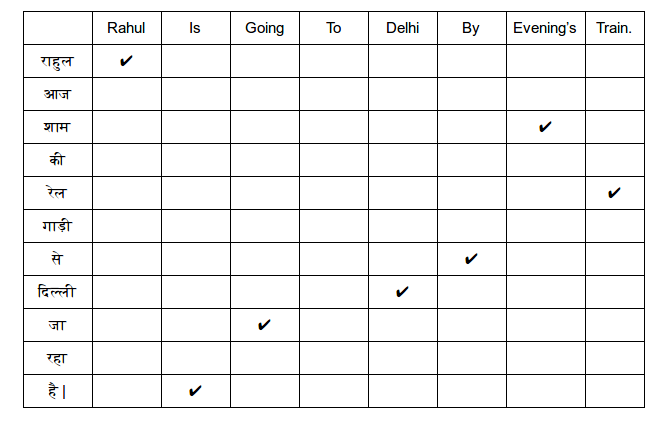
\includegraphics[scale=0.4]{Images/hindi_english}
        \caption{Alignment from Hindi to English}
        \label{fig:hindi_english}
\end{figure}
 A cell has \checkmark symbol if the row and column word are translation of each other. It is also possible that an entire row or column will not have \checkmark symbol, that's because there is no translation of that word in entire sentence. This is usually true for Articles and filler words.
\begin{figure}[H]
        \centering
        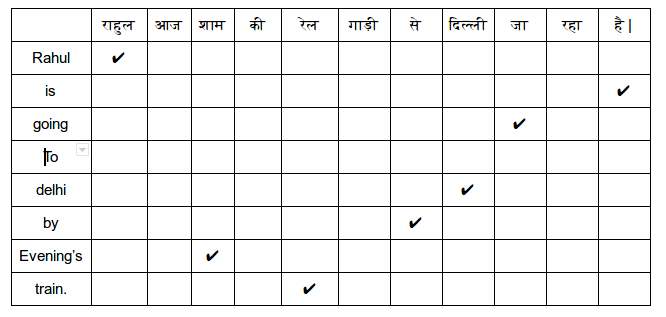
\includegraphics[scale=0.4]{Images/english_hindi}
        \caption{Alignment from English to Hindi}
        \label{fig:english_hindi}
\end{figure}
\subsection{Phrase construction}
Given word alignments, phrases are constructed as follows\cite{bhattacharyya,koehn}:
\begin{enumerate}
\item Every word of the sentence must be in some phrase.(Principle of coverage)
\item No empty phase is allowed. (Principal of Non-vacuousness).
\item All the words of language $L_{1}$ involved in a phrase must only align with words of language $L_{2}$ of the same phrase. (Principal of consistency)
\end{enumerate}
Figure \ref{fig:boxed} shows a possible phrases formed from the alignment phrases. Note that any given box will always follow the three principles of phrase construction. Figure \ref{fig:boxed_complete} shows bigger phrases formed using the  alignment figures \ref{fig:hindi_english} and \ref{fig:english_hindi}.
\begin{figure}[H]
        \centering
        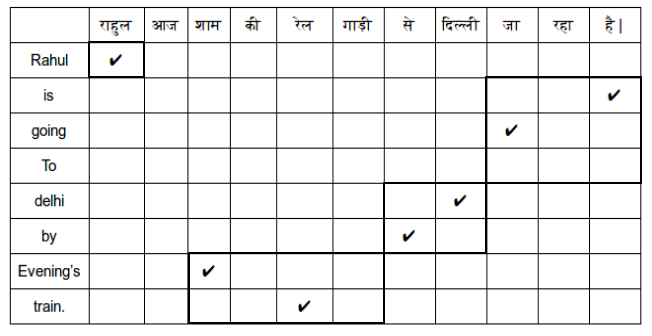
\includegraphics[scale=0.4]{Images/boxed.png}
        \caption{Few possible phrases from Alignments in figure \ref{fig:hindi_english} and \ref{fig:english_hindi}}
        \label{fig:boxed}
\end{figure}
\begin{figure}[H]
        \centering
        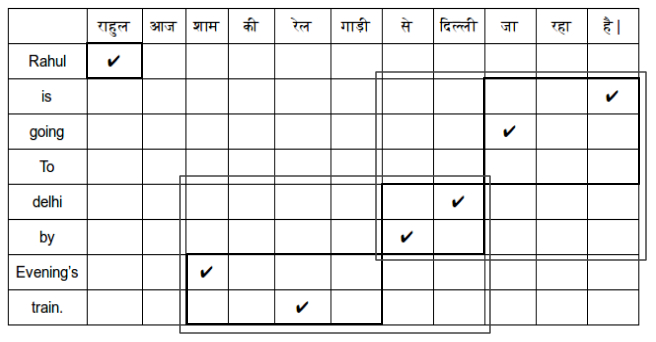
\includegraphics[scale=0.4]{Images/boxed_complete.png}
        \caption{Larger Phrases formed from figure \ref{fig:hindi_english} and \ref{fig:english_hindi}}
        \label{fig:boxed_complete}
\end{figure}

\section{Phrase Based SMT}
Phrase based SMT follows the same Noisy-channel model as
\begin{equation}
\hat{e} = arg max_{e}(P(e\mid f)) = arg max_{e}(P(e)\cdot(f\mid e))
\end{equation}
\begin{align}
P(f_{1}^{I}\mid e_{1}^{I}) &= P(f_{1},f_{2},\ldots,f_{I}\mid  e_{1},e_{2},\ldots,e_{I})\nonumber \\
		   &= \prod_{i=1}^{I}\Phi(f_{i}^{I}\mid e_{i}^{I})d(start_{i}-end{(i-1)}-1)
\end{align}

where LHS is the probability of $I$ phrases of $f$ given $I$ phrases of $e$ and RHS consists of two parts. The first part $\Phi$ is called the phrase translation probability, while the second part $d(\cdot)$ is called the distortion probability. 

\subsection{Estimating Phrase Translation and Distortion probability }
Phrase translation probability is found out by counting in how many sentences a particular phrase pair was extracted again all possible phrases of a English phrase.
\begin{equation}
\phi(f\mid e) = \frac{count(e,f)}{\sum_{f_{i}}count(e,f_{i})}
\end{equation}
Distortion probability is found out by simply for each phrase, calculating the difference in the position of the phrase in the input and translated sentence.
\begin{equation}
d(distance) = \frac{count(distance(\bar{e},\bar{f}))}{count(\bar{e})}
\end{equation}
The two candidate translation of \begin{hindi} फिर मिलेंगे, \end{hindi} \\
See you again.\\
Again see you, \\
will be decided using following parameters.
\begin{enumerate}
\item $P_{LM}(\text{see you again})$ and $P_{LM}(\text{see you again})$\\
\item $P(milenge\mid \text{see you})$ and $P(fir\mid again)$ \\
\item Distortion probability of $see you$ and $again$. 
\end{enumerate}








    
    \bibliographystyle{plain} 
    \bibliography{ref}
    
    

\end{document}
